\chapter{Introduction}
\label{chap:intro}
    %% TODO: put goals (requirements of a hardware DSL) before FP
    \acrodef{ILP}{Instruction-Level Paralellism}
    Several factors have been causing an increasing demand for hardware acceleration of algorithms.
    On the one hand, Moore's law still holds for the near future~\cite{itrs},
    which means bigger circuits in the same wafer area.
    On the other hand, advances in \ac{ILP} and microarchitecture of processors
    are starting to have diminishing returns~\cite{dark-silicon}.

    Also, there is pressure to reduce the duration and cost of the circuit design process.
    These trends are at odds with the techniques and tooling used in the hardware design process,
    which have not experienced the same evolution as the ones for software development.

    \acrodef{ASIC}{Application-Specific Integrated Circuit}
    The design of an \ac{ASIC} imposes strong requirements,
    specially with regards to correctness (functional and otherwise).
    Design mistakes which make their way into the manufacturing process can be very expensive,
    and errors that reach the consumer cost even more, as there's no such thing as "updating" a chip.
    One infamous example of such a bug reaching the consumer was the \emph{FDIV} bug in Intel's Pentium chip,
    which might have costed the company over 400 million dollars~\cite{intel-fdiv}.

    In the software industry, especially in application domains requiring high correctness assurance
    (such as information security, machine control, etc.),
    functional programming techniques have long been used to improve productivity
    and reduce the need for extensive testing and debugging.
    These claims have been confirmed both in industrial settings~\cite{haskell-productivity-wiger}
    and in experiments~\cite{haskell-productivity-hudak}.

    Another advantage usually attributed to functional programming is an increased capacity to
    \emph{reason} about your programs, specially to perform what is called \emph{equational reasoning}.
    Equational reasoning can be used even as an optimization technique.
    For example, some libraries for array programming in Haskell take advantage of the following
    law involving \texttt{map} and function composition.
    The proof is derived by structural induction on the array or list,
    and by using equational reasoning with the definitions of the functions involved:

    {\centering
        \begin{haskellcode}
            map f . map g == map (f . g)
        \end{haskellcode}
    }

    Besides the growing usage of functional programming languages in several domain areas,
    functional techniques and constructs keep "penetrating" imperative languages
    with each new release. Some examples are:

    \begin{itemize}
        \item Apple's recently released Swift™ language, which features immutable data structures,
            first-class functions and type inference.
        \item Java's adoption of \emph{generics} and – more recently – of lambda
            expressions\footnote{\url{http://docs.oracle.com/javase/tutorial/java/javaOO/lambdaexpressions.html}}.
        \item The concept of \emph{nullable type}\footnote{\url{http://msdn.microsoft.com/en-us/library/1t3y8s4s.aspx}}
            in C\#, equivalent to Haskell's \mintinline{haskell}{Maybe}.
        \item Python's \emph{generator expressions}, inspired by list comprehensions and lazy evaluation.
    \end{itemize}

    In a certain way, we can compare the power of the tools and techniques
    used nowadays in hardware design to the early days of software development.
    Of course there are inherent and fundamental differences between the two activities, but
    this comparison leads us to ask whether recent ideas from programming language research,
    specially those related to functional programming, can be used to improve hardware design.

    \acrodef{EDSL}{Embedded Domain-Specific Language}
    Research trying to answer this broad question started already in the 1980s,
    with the work of Prof. Mary Sheeran and others~\cite{sheeran-survey},
    developing \emph{functional} hardware description languages, such as \emph{μFP}~\cite{mufp-1984}.
    Later, a trend emerged of developing \acp{EDSL} for hardware description,
    \emph{hosted} in purely functional languages, such as Haskell~\cite{haskell2010}.
    Prominent examples of this trend are the Lava~\cite{lava-1999} family,
    as well as ForSyDe~\cite{forsyde1999}.

    A circuit description written in Lava – an \ac{EDSL} hosted in Haskell – can look like the following:

    \begin{haskellcode}
        toggle :: Signal Bool
        toggle = let output = inv (latch output) in output
    \end{haskellcode}

    Even though pure functional languages (especially Haskell) are well-suited for implementing \acp{EDSL},
    there is still room for improvement in the type-safety of the embedded languages.
    This can be done by hosting the \acp{EDSL} in a language supporting \emph{dependent types},
    as exemplified in the paper "The Power of Pi"~\cite{power-pi}.

    A type system with \emph{dependent types} can express strong properties about the programs written in it.
    Systems with dependent types can be seen as regular programming languages,
    but because of the expressive power of dependent types, we can also see them as \emph{interactive theorem provers}.

    \acrodef{DTP}{Dependently-Typed Programming}
    Using dependent types, one can more easily bring together \emph{specification} and \emph{implementation}.
    The type signature of a function can give many more \emph{guarantees} about its behaviour.
    A classical example when introducing \ac{DTP} is the type of statically-sized vectors,
    along with the safe \AF{head} function, depicted in Listing~\ref{lst:Vect-head}.

    \begin{listing}[h]
        \centering{\ExecuteMetaData[agda/latex/Report/ChapterIntroduction.tex]{Vect-head}}
        \caption{Type of sized vectors and the safe \AF{head} function. \label{lst:Vect-head}}
    \end{listing}

    In this example, the parameter to \AF{head} cannot be empty – its size will be at least 1 (\AI{suc} \AI{zero}).
    This is expressed in the parameter's type: \AD{Vect} \AB{α} (\AI{suc} \AB{n}).
    When checking the totality of \AF{head} (whether all cases are covered by pattern matching),
    the type checker will notice that the only constructor of \AD{Vect}
    able to produce an element of type \AD{Vect} \AB{α} (\AI{suc} \AB{n}) is \AI{\_∷\_}.

    In the safe \AF{head} example, we made the specification more precise by constraining the type of an argument.
    We can also use dependent types to make the return type of a function more precise.
    The \AF{group} function for sized vectors in \emph{Agda}'s standard library has the following type:

    \begin{center}
        \ExecuteMetaData[agda/latex/Report/ChapterIntroduction.tex]{group-decl}
    \end{center}

    It receives as parameters, besides the vector to be "sliced",
    the number of slices desired (\AB{n}) and the size of each slice (\AB{k}).
    Notice that the size of the passed vector needs to match (\AB{n} \AF{*} \AB{k}).
    The return type of this function may be read as:

    \begin{quote}
        A vector (\AB{xss}) of size \AB{n} (whose elements are vectors of size \AB{k}),
        such that \texttt{\AB{xs} \AF{≡} \AF{concat} \AB{xss}}.
    \end{quote}

    Therefore, it returns a collection of groups "sliced" from the original vector, each with the requested size.
    Additionally, it returns a proof that concatenating all groups results in the original vector.
    This type serves as a \emph{complete specification of correctness} for the function.
    Any function with this type is, by definition, a \emph{correct grouping function}.

    \acrodef{DSL}{Domain-Specific Language}
    In a deep-embedded \acs{DSL} for hardware there is usually a \emph{type} representing circuits.
    One can imagine that it would be useful to design this type
    in such a way that as few of its elements as possible are \emph{malformed}.
    Therefore, we want to make the typing of the circuits as strong as possible,
    to eliminate as many \emph{classes of design mistakes} as possible.

    Depedent type systems allow for easy expression of these \emph{well-formedness} rules for circuits.
    One simple criterion of circuit \emph{well-formedness} is, for example, that it contains no \emph{floating} signals.
    That is, all of a circuit's internal components must have all their ports connected.
    Figure~\ref{fig:floating-wire} shows an example of circuit violating this rule.

    \begin{figure}[h]
        \centering{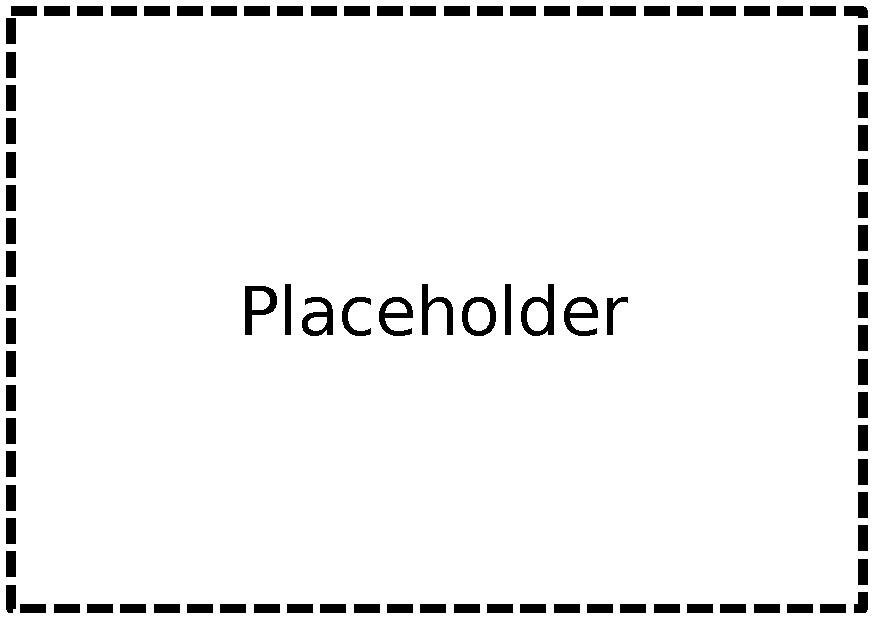
\includegraphics[width=0.3\textwidth]{imgs/floating-wire.pdf}}
        \caption{Malformed circuit with a \emph{floating} signal. \label{fig:floating-wire}}
    \end{figure}

    \acrodef{VHDL}{VHSIC Hardware Description Language}
    In this M.Sc thesis we developed a hardware \ac{EDSL} – Π-Ware – which enforces this and other
    well-formedness rules using dependent types.
    Π-Ware is a \emph{deep-embedded} \ac{DSL} hosted in the Agda programming language,
    supporting simulation for combinational and synchronous sequential circuits.
    Furthermore, the user of Π-Ware can prove \emph{expressive} properties about circuits in the logic
    of Agda itself (intuitionistic logic).

    In Chapter~\ref{chap:background} we will establish the questions, concepts, languages and tools
    from which we took inspiration to create Π-Ware.
    We will discuss the process of hardware design, functional languages for hardware,
    and how dependent types can enter the picture.

    In Chapter~\ref{chap:piware} we dive into a detailed study of the Π-Ware \ac{EDSL} itself.
    We provide a detailed account of how Π-Ware works currently,
    what design decisions were involved in its development, and how to use it.
    We give examples of circuits modelled in Π-Ware and proofs of properties involving
    these circuits.

    Finally, in Chapter~\ref{chap:conclusions}, we discuss what has been achieved by Π-Ware as it stands
    by comparing it with other hardware \acp{EDSL}, recent and past.
    We also clarify what desirable features reamin to be implemented as future work,
    and on which conditions (if any) these implementation efforts depend.

